\documentclass[border=6pt,tikz]{standalone}
\usepackage{tikz}
\usepackage{amsmath,amssymb}
\usetikzlibrary{arrows.meta,positioning,fit,backgrounds,calc,shapes.geometric,decorations.pathreplacing,patterns}
\definecolor{ink}{HTML}{1B2430}
\definecolor{muted}{HTML}{6B7785}
\definecolor{accent}{HTML}{2F6FB5}
\definecolor{accent2}{HTML}{C1611F}
\definecolor{good}{HTML}{2E7D5B}
\definecolor{soft}{HTML}{EDF2F7}
\definecolor{soft2}{HTML}{FBEDE2}
\definecolor{soft3}{HTML}{E6F0E9}
\tikzset{
  box/.style={draw=ink,line width=.7pt,rounded corners=2pt,fill=soft,inner sep=4pt,align=center,font=\sffamily\small},
  boxa/.style={box,fill=soft2},
  boxb/.style={box,fill=soft3},
  plain/.style={align=center,font=\sffamily\small,text=ink},
  tiny/.style={align=center,font=\sffamily\scriptsize,text=muted},
  ar/.style={-{Stealth[length=2.4mm]},draw=ink,line width=.7pt},
  arm/.style={-{Stealth[length=2.4mm]},draw=muted,line width=.6pt,dashed},
  nd/.style={circle,draw=ink,line width=.7pt,fill=white,minimum size=7mm,inner sep=0pt,font=\sffamily\scriptsize},
  ndf/.style={nd,fill=soft},
  ndt/.style={nd,fill=soft2},
}

\begin{document}
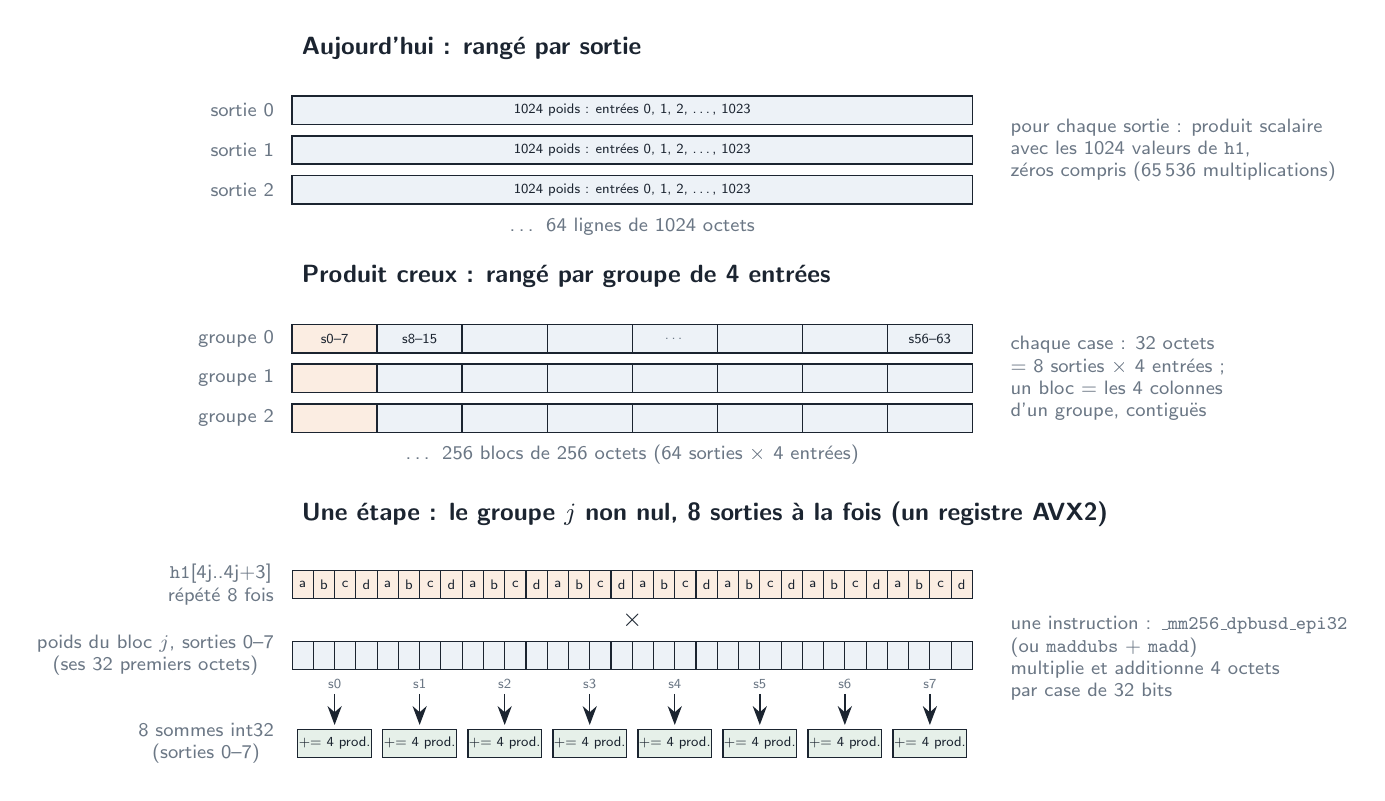
\begin{tikzpicture}[x=3.6mm,y=3.6mm]
  % ── today: row-major, one row per output ──
  \node[plain,anchor=west,font=\sffamily\small\bfseries] at (0,13.2) {Aujourd'hui : rangé par sortie};
  \foreach \r/\lab in {0/{sortie 0},1/{sortie 1},2/{sortie 2}} {
    \draw[ink,line width=.5pt,fill=soft] (0,10.5-1.4*\r) rectangle ++(24,1);
    \node[font=\sffamily\tiny,text=ink] at (12,11-1.4*\r) {1024 poids : entrées 0, 1, 2, …, 1023};
    \node[tiny,anchor=east] at (-.3,11-1.4*\r) {\lab};
  }
  \node[tiny] at (12,6.9) {… 64 lignes de 1024 octets};
  \node[tiny,anchor=west,align=left] at (25,9.6) {pour chaque sortie : produit scalaire\\avec les 1024 valeurs de \texttt{h1},\\zéros compris (65\,536 multiplications)};

  % ── sparse: by groups of 4 inputs ──
  \begin{scope}[yshift=-29mm]
  \node[plain,anchor=west,font=\sffamily\small\bfseries] at (0,13.2) {Produit creux : rangé par groupe de 4 entrées};
  \foreach \r/\lab in {0/{groupe 0},1/{groupe 1},2/{groupe 2}} {
    \draw[ink,line width=.5pt,fill=soft2] (0,10.5-1.4*\r) rectangle ++(3,1);
    \foreach \o in {1,...,7} {
      \draw[ink,line width=.5pt,fill=soft] (3*\o,10.5-1.4*\r) rectangle ++(3,1);
    }
    \node[tiny,anchor=east] at (-.3,11-1.4*\r) {\lab};
  }
  \node[font=\sffamily\tiny,text=ink] at (1.5,11) {s0–7};
  \node[font=\sffamily\tiny,text=ink] at (4.5,11) {s8–15};
  \node[font=\sffamily\tiny,text=ink] at (22.5,11) {s56–63};
  \node[font=\sffamily\tiny,text=muted] at (13.5,11) {…};
  \node[tiny] at (12,6.9) {… 256 blocs de 256 octets (64 sorties × 4 entrées)};
  \node[tiny,anchor=west,align=left] at (25,9.6) {chaque case : 32 octets\\= 8 sorties × 4 entrées ;\\un bloc = les 4 colonnes\\d'un groupe, contiguës};
  \end{scope}

  % ── one step of the sparse product, zoomed ──
  \begin{scope}[yshift=-57mm]
  \node[plain,anchor=west,font=\sffamily\small\bfseries] at (0,12.6) {Une étape : le groupe \(j\) non nul, 8 sorties à la fois (un registre AVX2)};
  % broadcast of 4 bytes
  \foreach \l in {0,...,7} {
    \foreach \t/\c in {0/a,1/b,2/c,3/d} \draw[ink,line width=.4pt,fill=soft2] (3*\l+.75*\t,9.6) rectangle ++(.75,1) node[midway,font=\sffamily\tiny]{\c};
  }
  \node[tiny,anchor=east] at (-.3,10.1) {\texttt{h1}[4j..4j+3]\\répété 8 fois};
  \node[plain] at (12,8.85) {\(\times\)};
  \foreach \l in {0,...,7} {
    \foreach \t in {0,...,3} \draw[ink,line width=.4pt,fill=soft] (3*\l+.75*\t,7.1) rectangle ++(.75,1);
    \node[font=\sffamily\tiny,text=muted] at (3*\l+1.5,6.6) {s\l};
  }
  \node[tiny,anchor=east] at (-.3,7.6) {poids du bloc \(j\), sorties 0–7\\(ses 32 premiers octets)};
  \foreach \l in {0,...,7} \draw[ar,line width=.5pt] (3*\l+1.5,6.25) -- (3*\l+1.5,5.15);
  \foreach \l in {0,...,7} \draw[ink,line width=.5pt,fill=soft3] (3*\l+.2,4) rectangle ++(2.6,1) node[midway,font=\sffamily\tiny]{+= 4 prod.};
  \node[tiny,anchor=east] at (-.3,4.5) {8 sommes int32\\(sorties 0–7)};
  \node[tiny,anchor=west,align=left] at (25,7.5) {une instruction : \texttt{\_mm256\_dpbusd\_epi32}\\(ou \texttt{maddubs} + \texttt{madd})\\multiplie et additionne 4 octets\\par case de 32 bits};
  \end{scope}
\end{tikzpicture}
\end{document}
